\documentclass[border=3pt]{standalone}
% Preâmbulo compartilhado pelos diagramas TikZ da aula 12 (Mapeamento por Grade de Ocupação)
\usepackage[T1]{fontenc}
\usepackage[utf8]{inputenc}
\usepackage{lmodern}
\usepackage{amsmath}
\usepackage{xcolor}
\usepackage{tikz}
\usetikzlibrary{arrows.meta,angles,quotes,decorations.pathmorphing,calc,
                positioning,shapes.geometric,shapes.misc,backgrounds,fit,
                math}

% Paleta (mesma dos SVGs originais)
\definecolor{dblue}{HTML}{2A5B8C}
\definecolor{dorange}{HTML}{B3541E}
\definecolor{dgreen}{HTML}{4A7C59}
\definecolor{dred}{HTML}{9C4B4B}
\definecolor{dcream}{HTML}{F4F1EA}
\definecolor{dshade}{HTML}{DDD7C9}

% Função gaussiana (não normalizada por padrão de escala visual)
\pgfmathdeclarefunction{gauss}{3}{%
  \pgfmathparse{1/(#3*sqrt(2*pi))*exp(-((#1-#2)^2)/(2*#3^2))}%
}

% Estilos comuns (prefixo d... para não colidir com chaves internas do pgf)
\tikzset{
  >={Stealth[length=2mm]},
  dguide/.style={gray!55, dashed, line width=0.4pt},
  daxis/.style={gray!60, line width=0.7pt, ->},
  dbody/.style={fill=black!3, draw=black!80, line width=1pt},
  dacc/.style={draw=dblue, line width=1pt},
  dlbl/.style={black!55, font=\small},
  dsub/.style={black!45, font=\footnotesize},
  dstate/.style={circle, draw=black!80, fill=dcream, line width=1pt,
                 minimum size=17mm, font=\large, inner sep=1pt},
  dobs/.style={circle, draw=black!80, fill=dshade, line width=1pt,
               minimum size=14mm, font=\large, inner sep=1pt},
  dbox/.style={rounded corners=2pt, draw=black!80, fill=dcream, line width=1pt,
               align=center, inner sep=6pt},
  dop/.style={circle, draw=black!80, fill=white, line width=1pt,
              minimum size=6mm, inner sep=0pt, font=\small},
  dtrans/.style={->, dblue, line width=1pt},
  dmeas/.style={->, dorange, line width=1pt},
  dcurve/.style={line width=1pt, dblue},
  dcurveb/.style={line width=1.4pt, dorange},
}

\begin{document}
\hyphenpenalty=10000 \exhyphenpenalty=10000 \tolerance=9999 \emergencystretch=3em
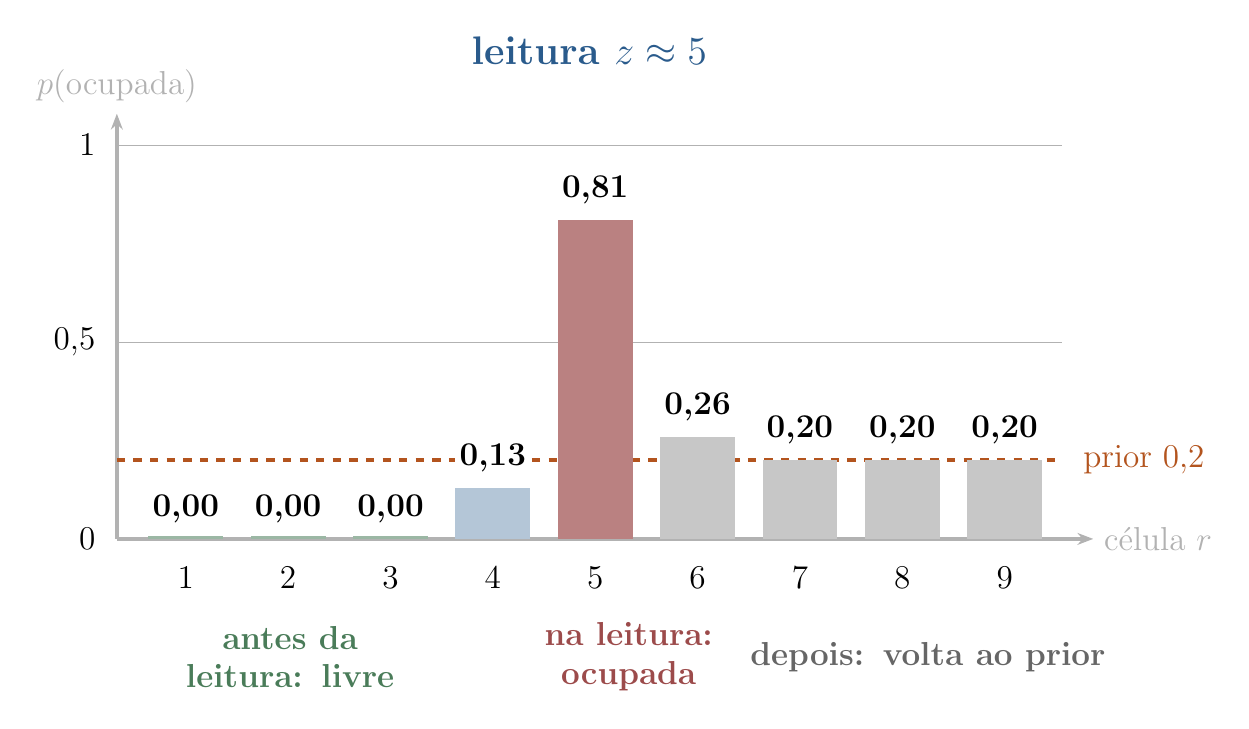
\begin{tikzpicture}[x=1cm,y=1cm]
\draw[daxis, line width=1.2pt] (0,0) -- (12.4,0) node[right, font=\large] {célula $r$};
  \draw[daxis, line width=1.2pt] (0,0) -- (0,5.4) node[above, font=\large] {$p(\text{ocupada})$};
  \draw[black!30, line width=0.4pt] (0,0.0) -- (12.0,0.0);
  \node[font=\large, anchor=east] at (-0.15,0.0) {0};
  \draw[black!30, line width=0.4pt] (0,2.5) -- (12.0,2.5);
  \node[font=\large, anchor=east] at (-0.15,2.5) {0,5};
  \draw[black!30, line width=0.4pt] (0,5.0) -- (12.0,5.0);
  \node[font=\large, anchor=east] at (-0.15,5.0) {1};
  \draw[dorange, dashed, line width=1.6pt] (0,1.0) -- (12.0,1.0);
  \node[font=\large, dorange, anchor=west] at (12.15,1.0) {prior $0{,}2$};
  \fill[dgreen!55] (0.4,0) rectangle (1.35,0.04);
  \node[font=\large\bfseries, fill=white, inner sep=1.5pt] at (0.875,0.38) {0,00};
  \node[font=\large] at (0.875,-0.5) {1};
  \fill[dgreen!55] (1.7000000000000002,0) rectangle (2.65,0.04);
  \node[font=\large\bfseries, fill=white, inner sep=1.5pt] at (2.175,0.38) {0,00};
  \node[font=\large] at (2.175,-0.5) {2};
  \fill[dgreen!55] (3.0,0) rectangle (3.95,0.04);
  \node[font=\large\bfseries, fill=white, inner sep=1.5pt] at (3.475,0.38) {0,00};
  \node[font=\large] at (3.475,-0.5) {3};
  \fill[dblue!35] (4.300000000000001,0) rectangle (5.25,0.65);
  \node[font=\large\bfseries, fill=white, inner sep=1.5pt] at (4.775,1.03) {0,13};
  \node[font=\large] at (4.775,-0.5) {4};
  \fill[dred!70] (5.6000000000000005,0) rectangle (6.55,4.05);
  \node[font=\large\bfseries, fill=white, inner sep=1.5pt] at (6.075,4.43) {0,81};
  \node[font=\large] at (6.075,-0.5) {5};
  \fill[black!22] (6.9,0) rectangle (7.85,1.3);
  \node[font=\large\bfseries, fill=white, inner sep=1.5pt] at (7.375,1.68) {0,26};
  \node[font=\large] at (7.375,-0.5) {6};
  \fill[black!22] (8.200000000000001,0) rectangle (9.15,1.0);
  \node[font=\large\bfseries, fill=white, inner sep=1.5pt] at (8.675,1.38) {0,20};
  \node[font=\large] at (8.675,-0.5) {7};
  \fill[black!22] (9.5,0) rectangle (10.45,1.0);
  \node[font=\large\bfseries, fill=white, inner sep=1.5pt] at (9.975,1.38) {0,20};
  \node[font=\large] at (9.975,-0.5) {8};
  \fill[black!22] (10.8,0) rectangle (11.75,1.0);
  \node[font=\large\bfseries, fill=white, inner sep=1.5pt] at (11.275,1.38) {0,20};
  \node[font=\large] at (11.275,-0.5) {9};
  \node[font=\large\bfseries, dgreen, text width=4cm, align=center] at (2.2,-1.5) {antes da leitura: \textbf{livre}};
  \node[font=\large\bfseries, dred, text width=4cm, align=center] at (6.5,-1.5) {na leitura: \textbf{ocupada}};
  \node[font=\large\bfseries, black!60, text width=5cm, align=center] at (10.3,-1.5) {depois: volta ao \textbf{prior}};
  \node[font=\Large\bfseries, dblue] at (6.0,6.2) {leitura $z \approx 5$};
\end{tikzpicture}
\end{document}
